\documentclass[10pt,aspectratio=43]{beamer}

\usepackage{graphicx}
\usepackage{tikz}
\usepackage{xcolor}
\usepackage{caption}
\usepackage{subcaption}
\usepackage{bm}
\usetikzlibrary{calc} 
\usepackage{hyperref}
\hypersetup{
    colorlinks=true,
    linkcolor=blue,
    urlcolor=red
}
\usepackage{fontawesome5}
\usepackage{ulem}

\usetheme{MyStyle}   % loads beamerthemeMyStyle.sty
\setlength{\columnsep}{0pt}


%%%%%%%%%%%%%%%%%%%%%%%%%%%%%%%%%%%%%%%%%%
%%%%%%%%%%%%%%%%%%%%%%%%%%%%%%%%%%%%%%%%%%
%%%%%%%%%%%%%%%%%%%%%%%%%%%%%%%%%%%%%%%%%%

\title{Time calibration}
\newcommand{\eventname}{ALERT reconstruction}
\author{Felix Touchte Codjo}
\institute{IJCLab}
\date{\today}


\begin{document}

\begin{frame}[plain] % remove header, footer, barre de navigation
\titlepage
\end{frame}

%\begin{frame}{Outline}
%\tableofcontents
%\end{frame}

%\section{Intro}
% \section{Updates}

\begin{frame}{Time calibration}
    \begin{itemize} \scriptsize %\footnotesize
        \item Residuals and T2D distributions with the current (on the left) and old (on the right) t0 and T2D tables
        \item The old distributions are obtained using this timestamp : May 23, 2026
        \item Both distributions are obtained using coatjava development. The run number is 22712 and the elastic cuts are $3.5 < W^2 < 3.8 \mbox{ GeV}^2$, $|\Delta \phi| < 20^\circ$, nb hits per track $\ge 6$
    \end{itemize}

    \centering
    \vspace{0.1cm}

    % 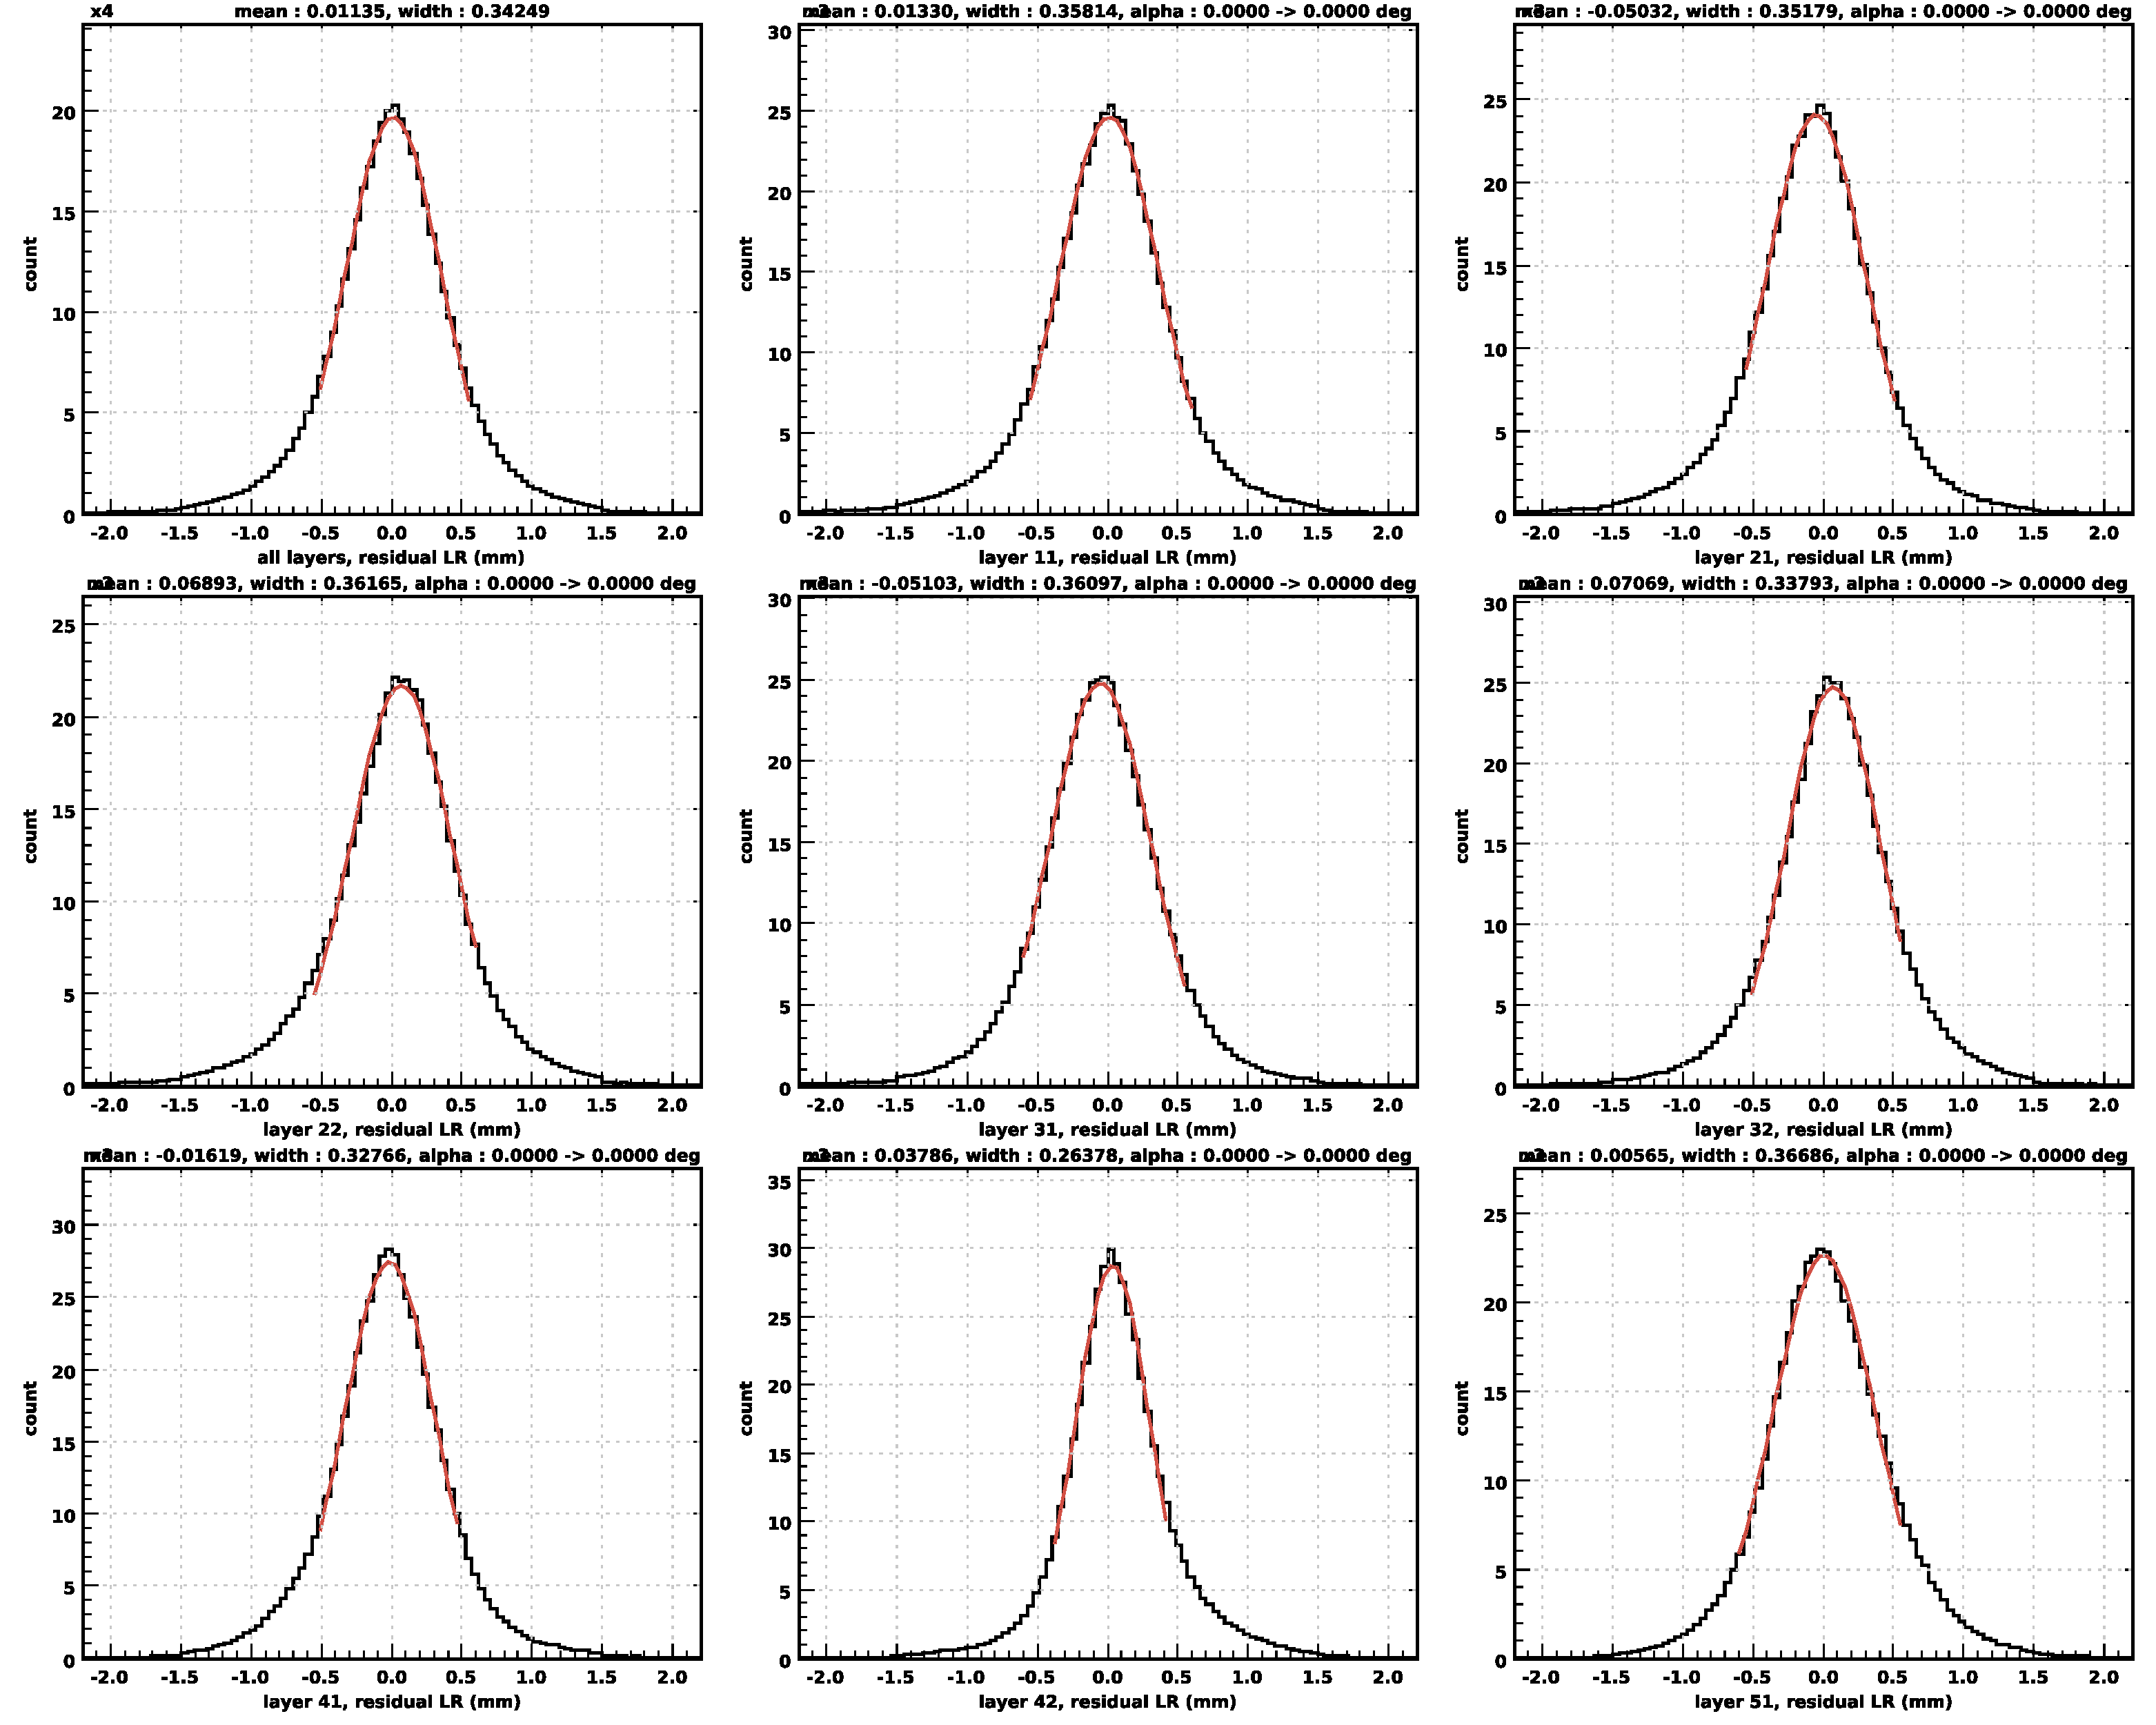
\includegraphics[width=0.7\linewidth]{figures/residual_LR_iter_1_before.pdf}

    \begin{tabular}{cc}
        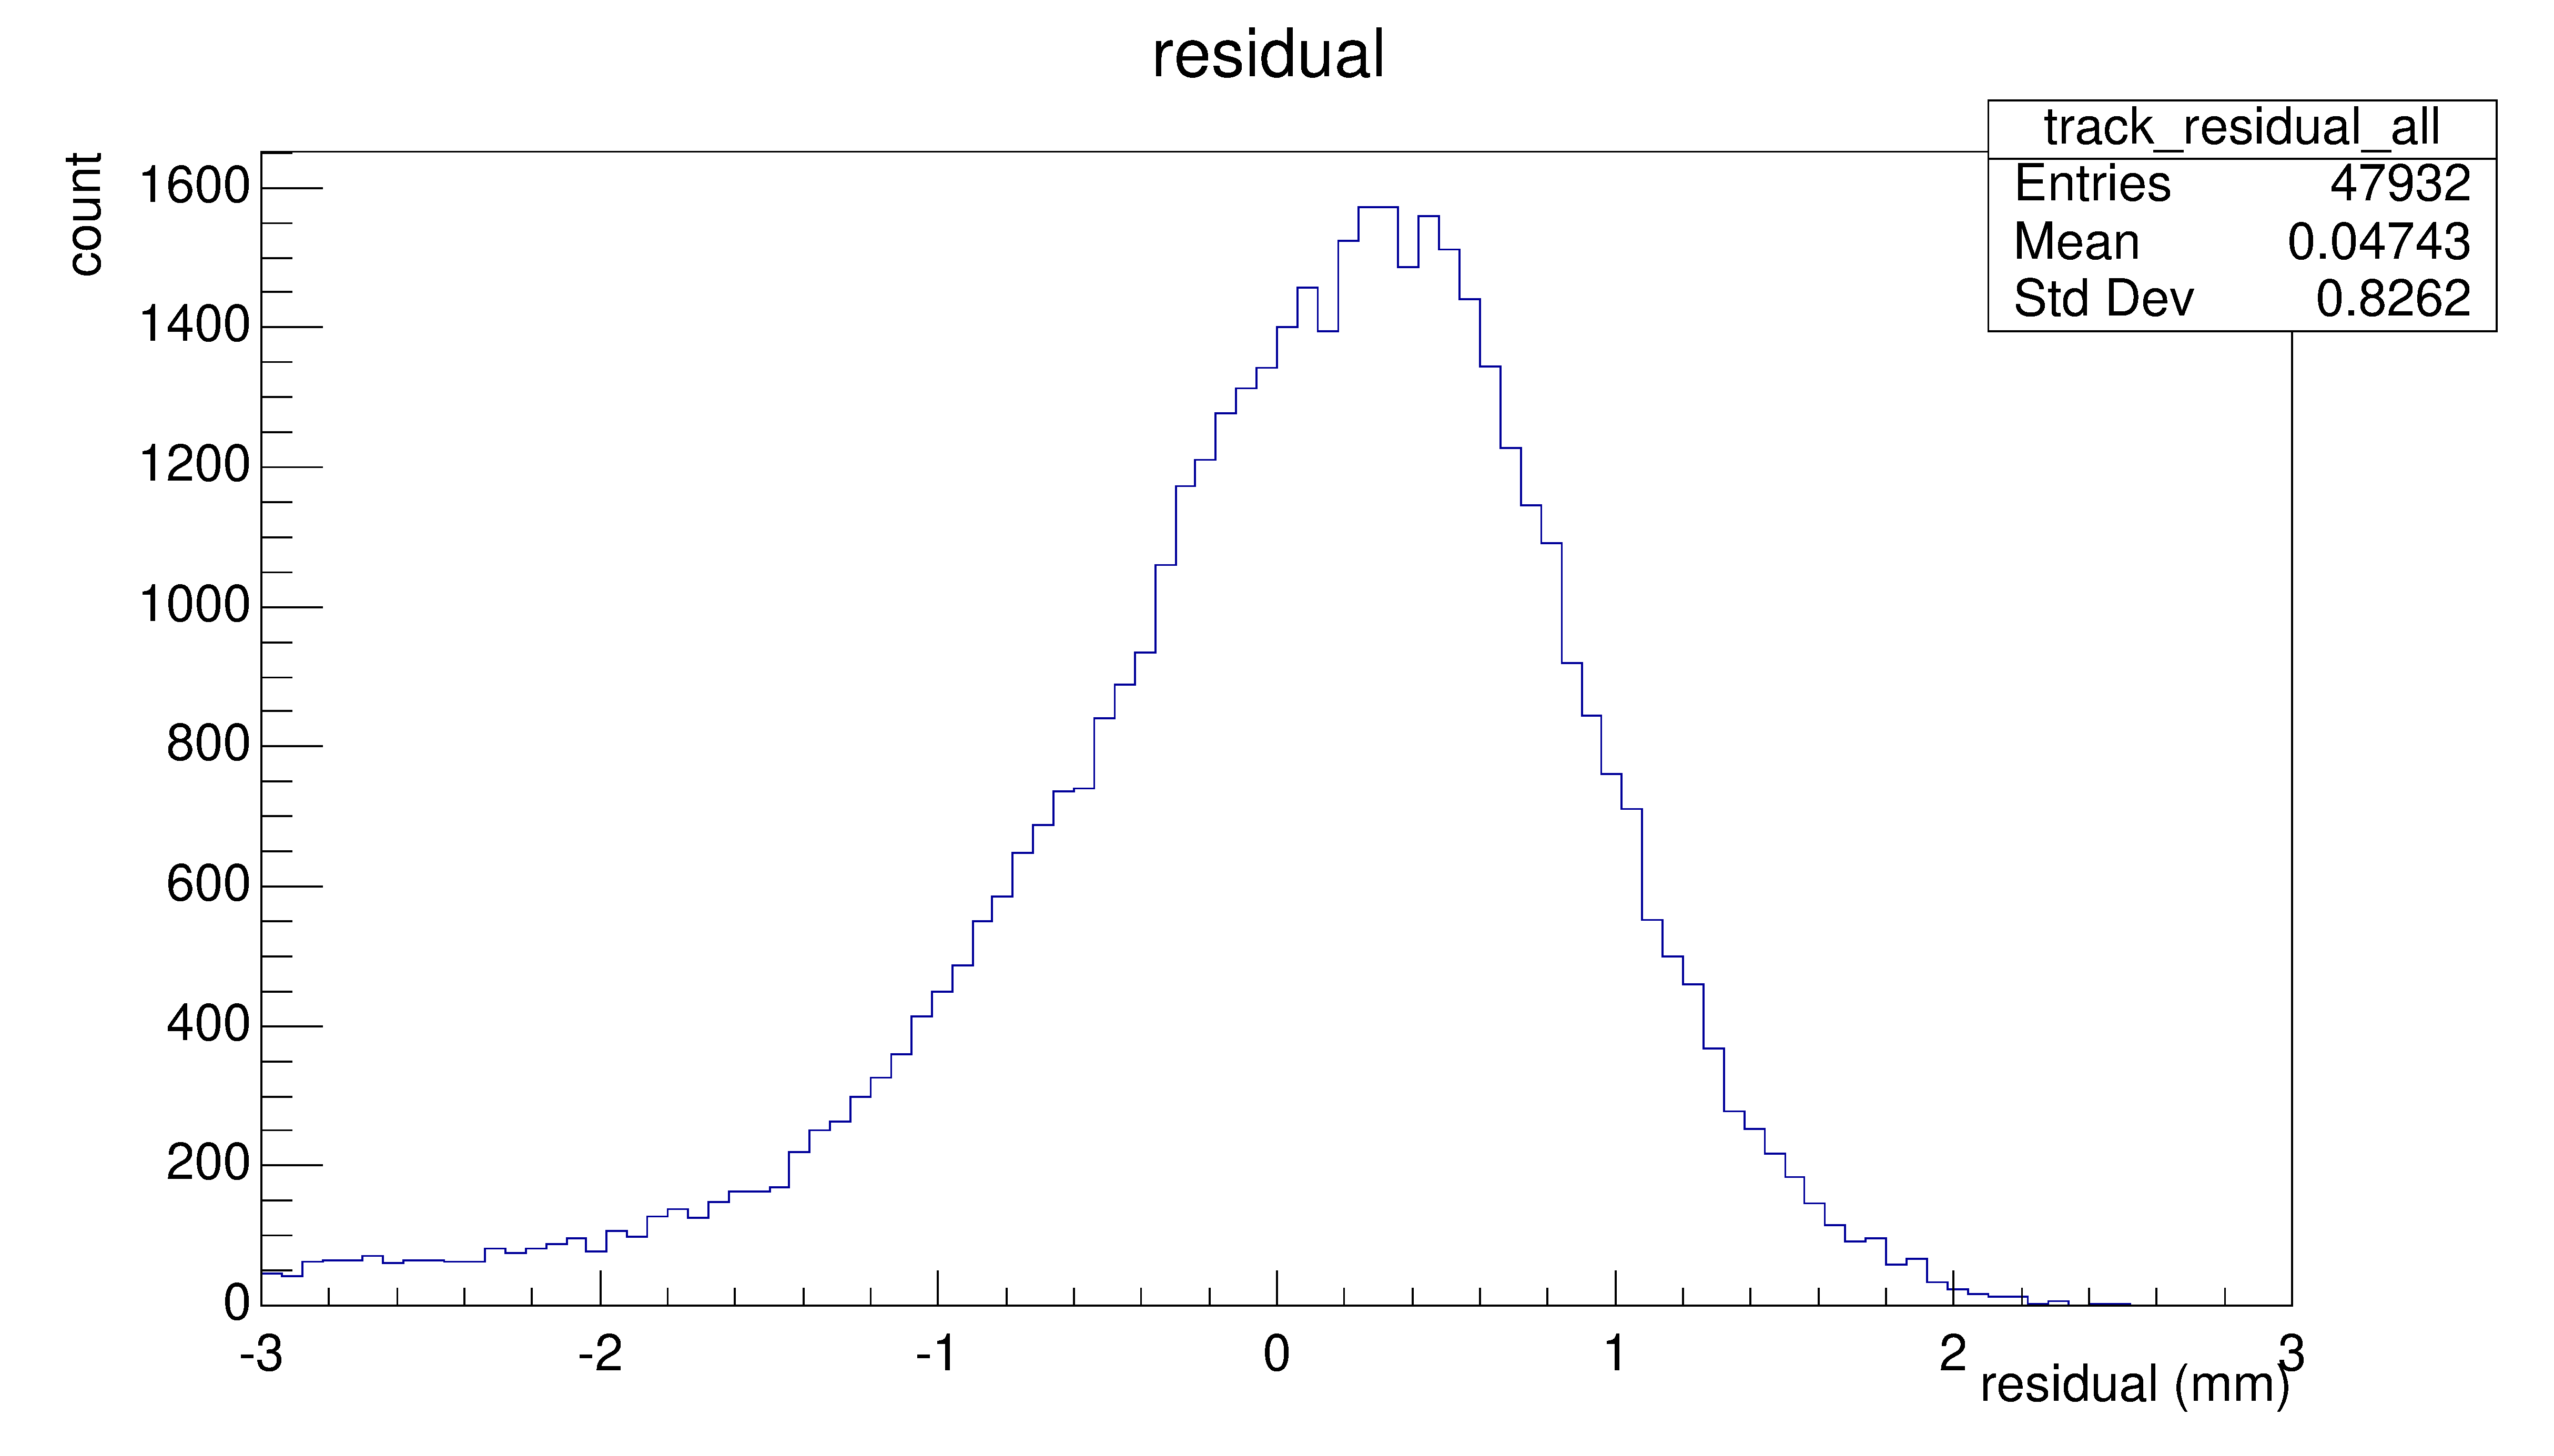
\includegraphics[width=0.45\linewidth]{figures/new_residuals.pdf} & 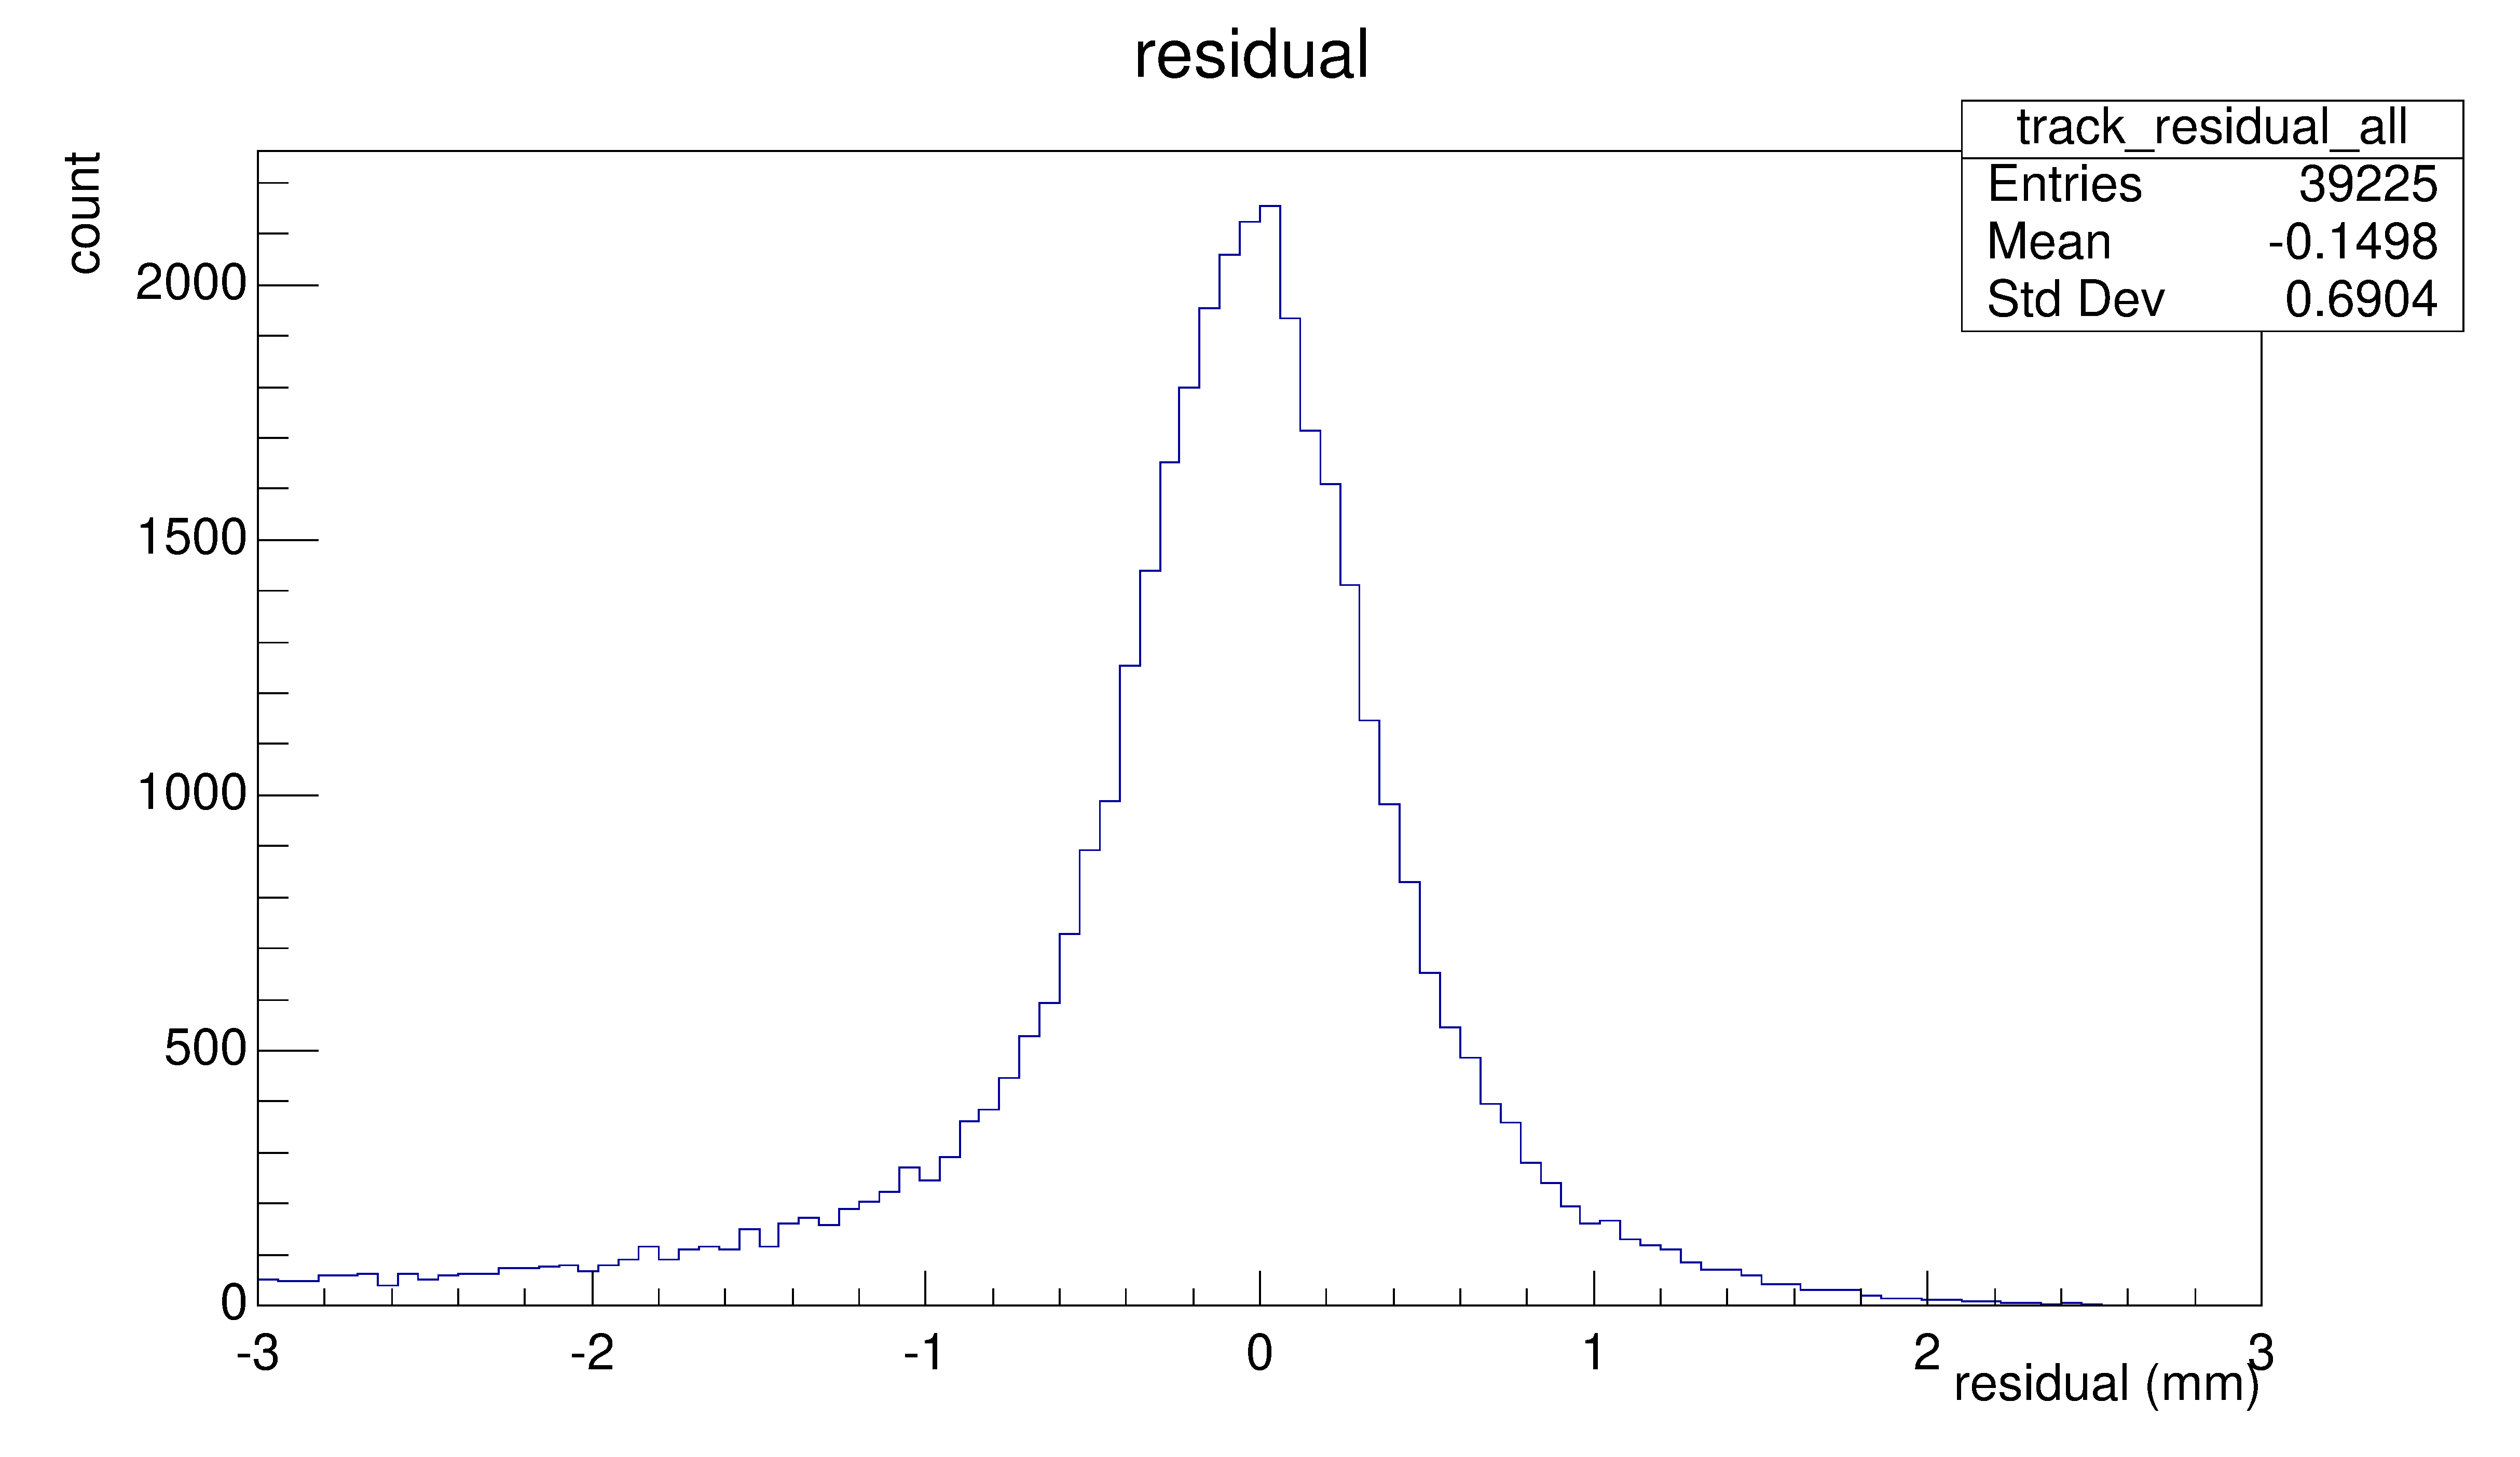
\includegraphics[width=0.45\linewidth]{figures/old_residuals.pdf} \\
        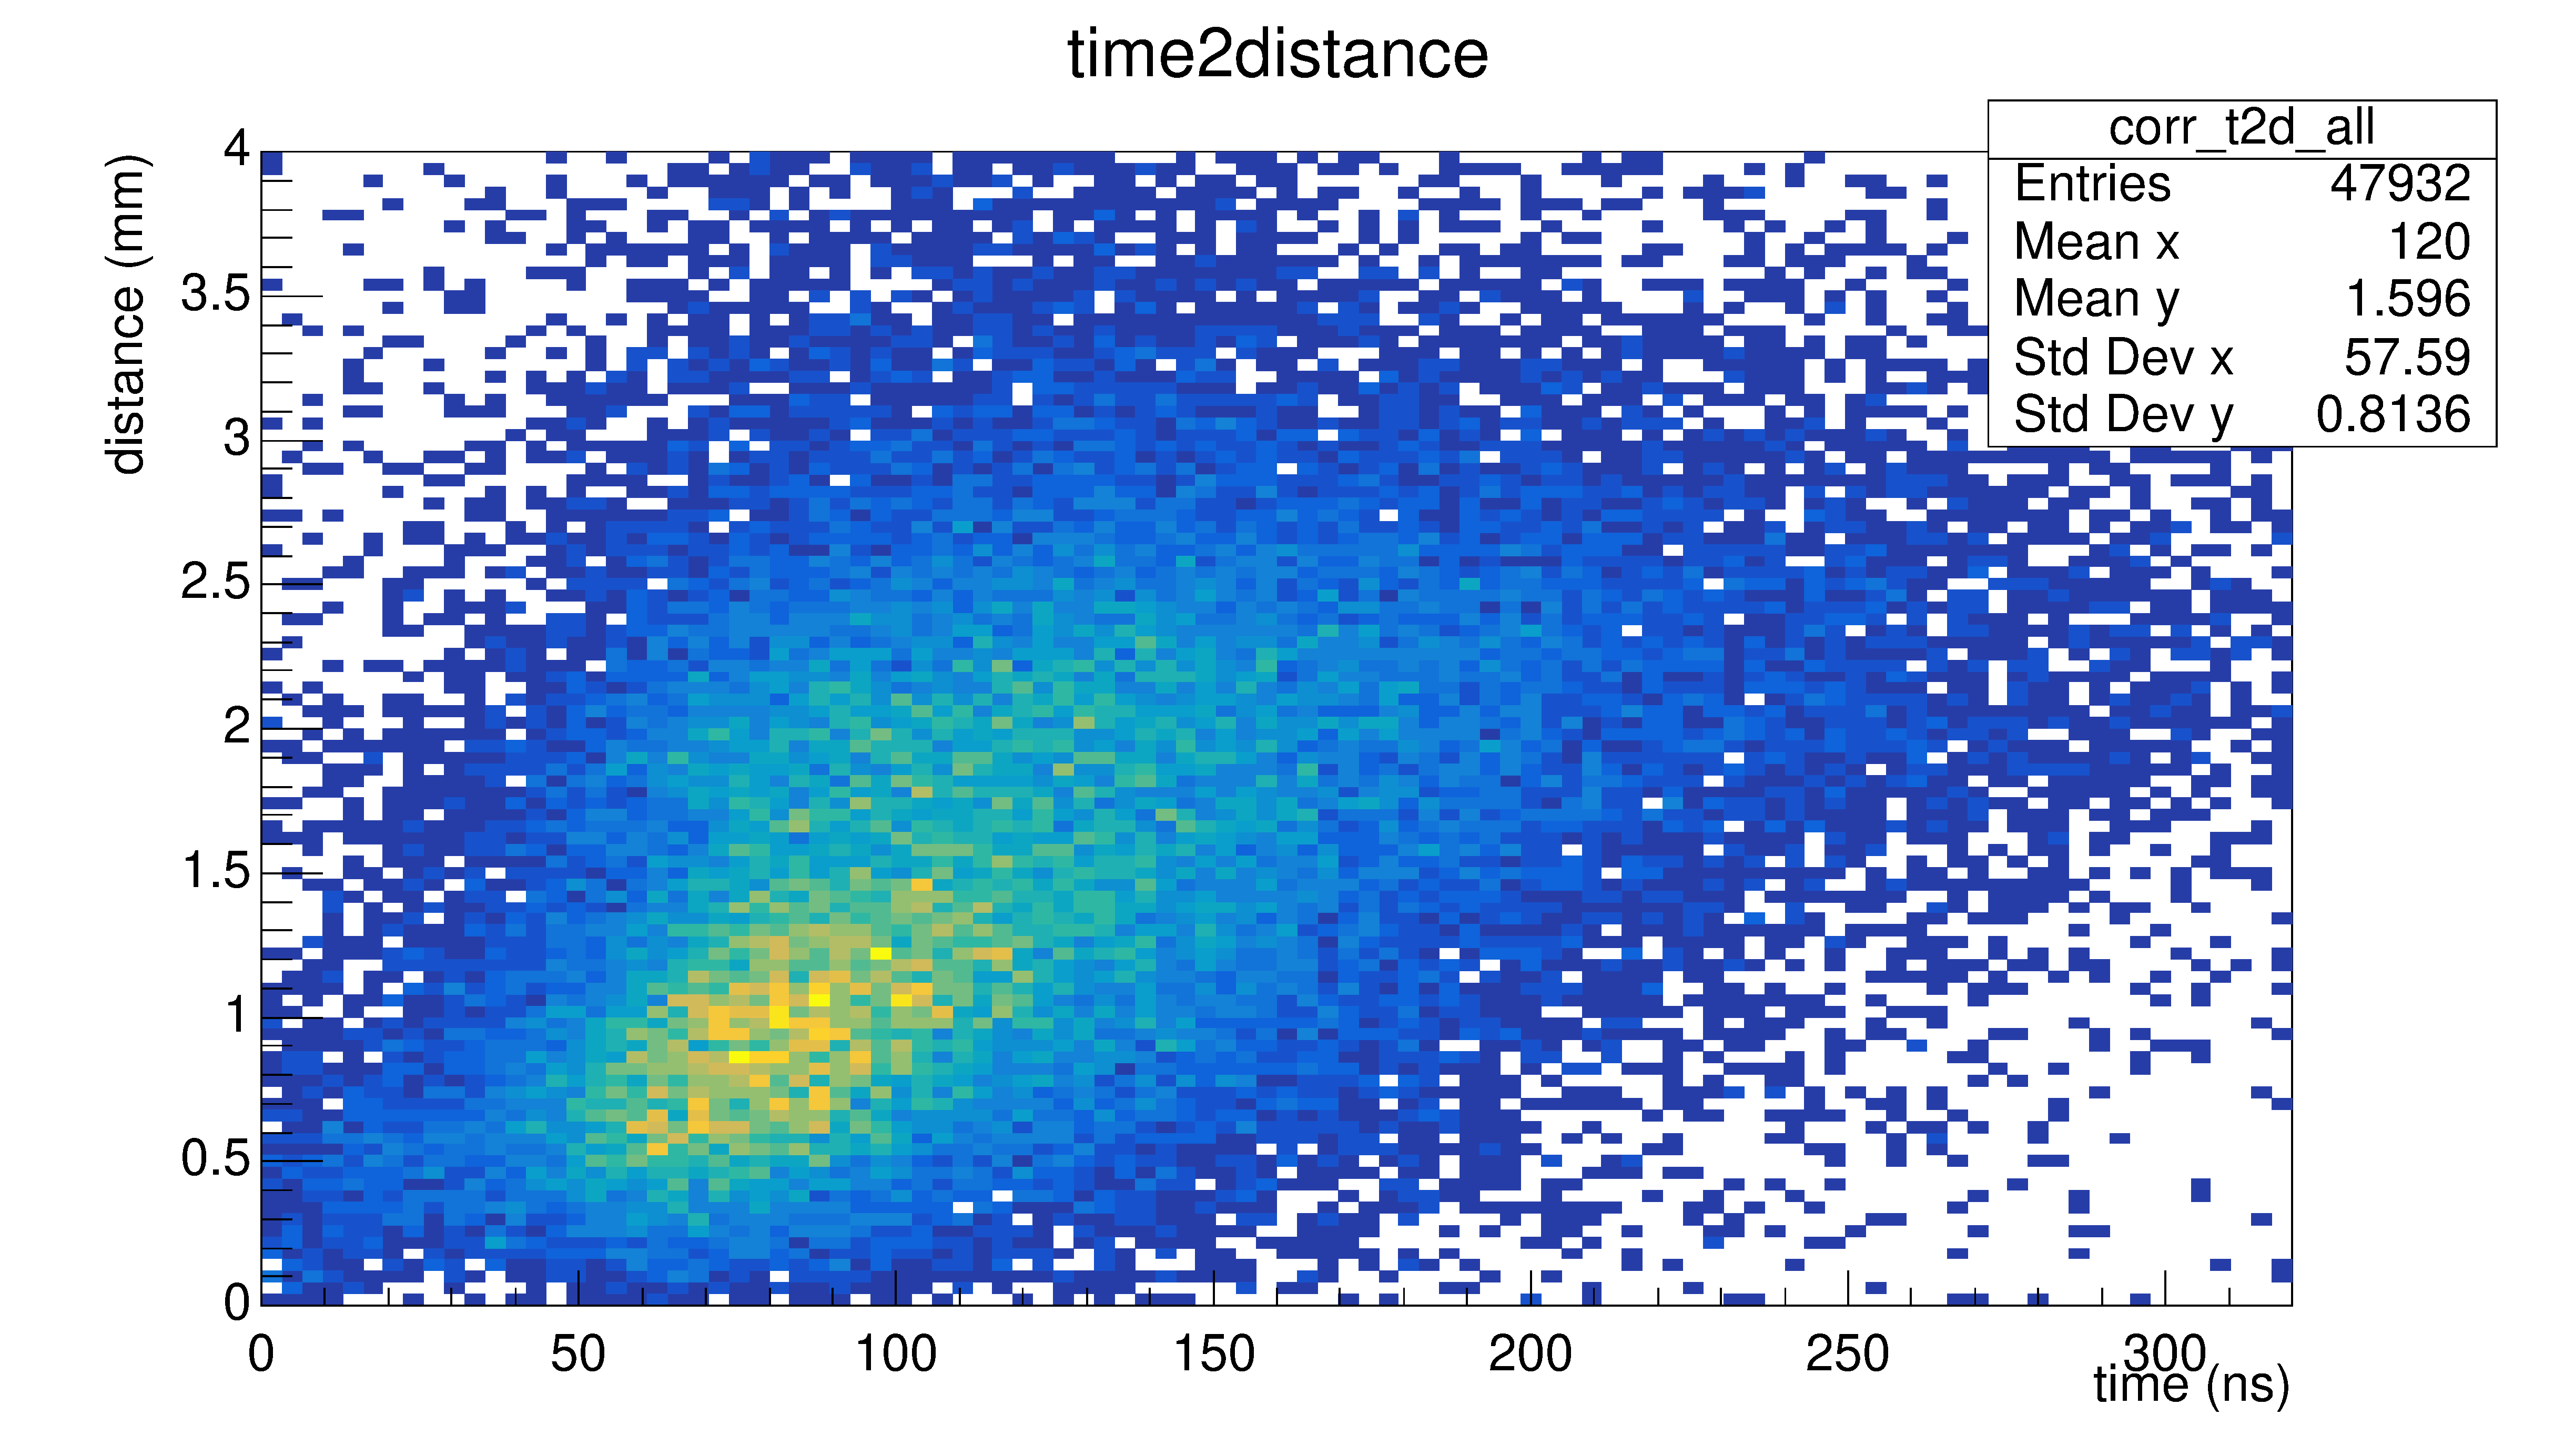
\includegraphics[width=0.45\linewidth]{figures/new_t2d.pdf} & 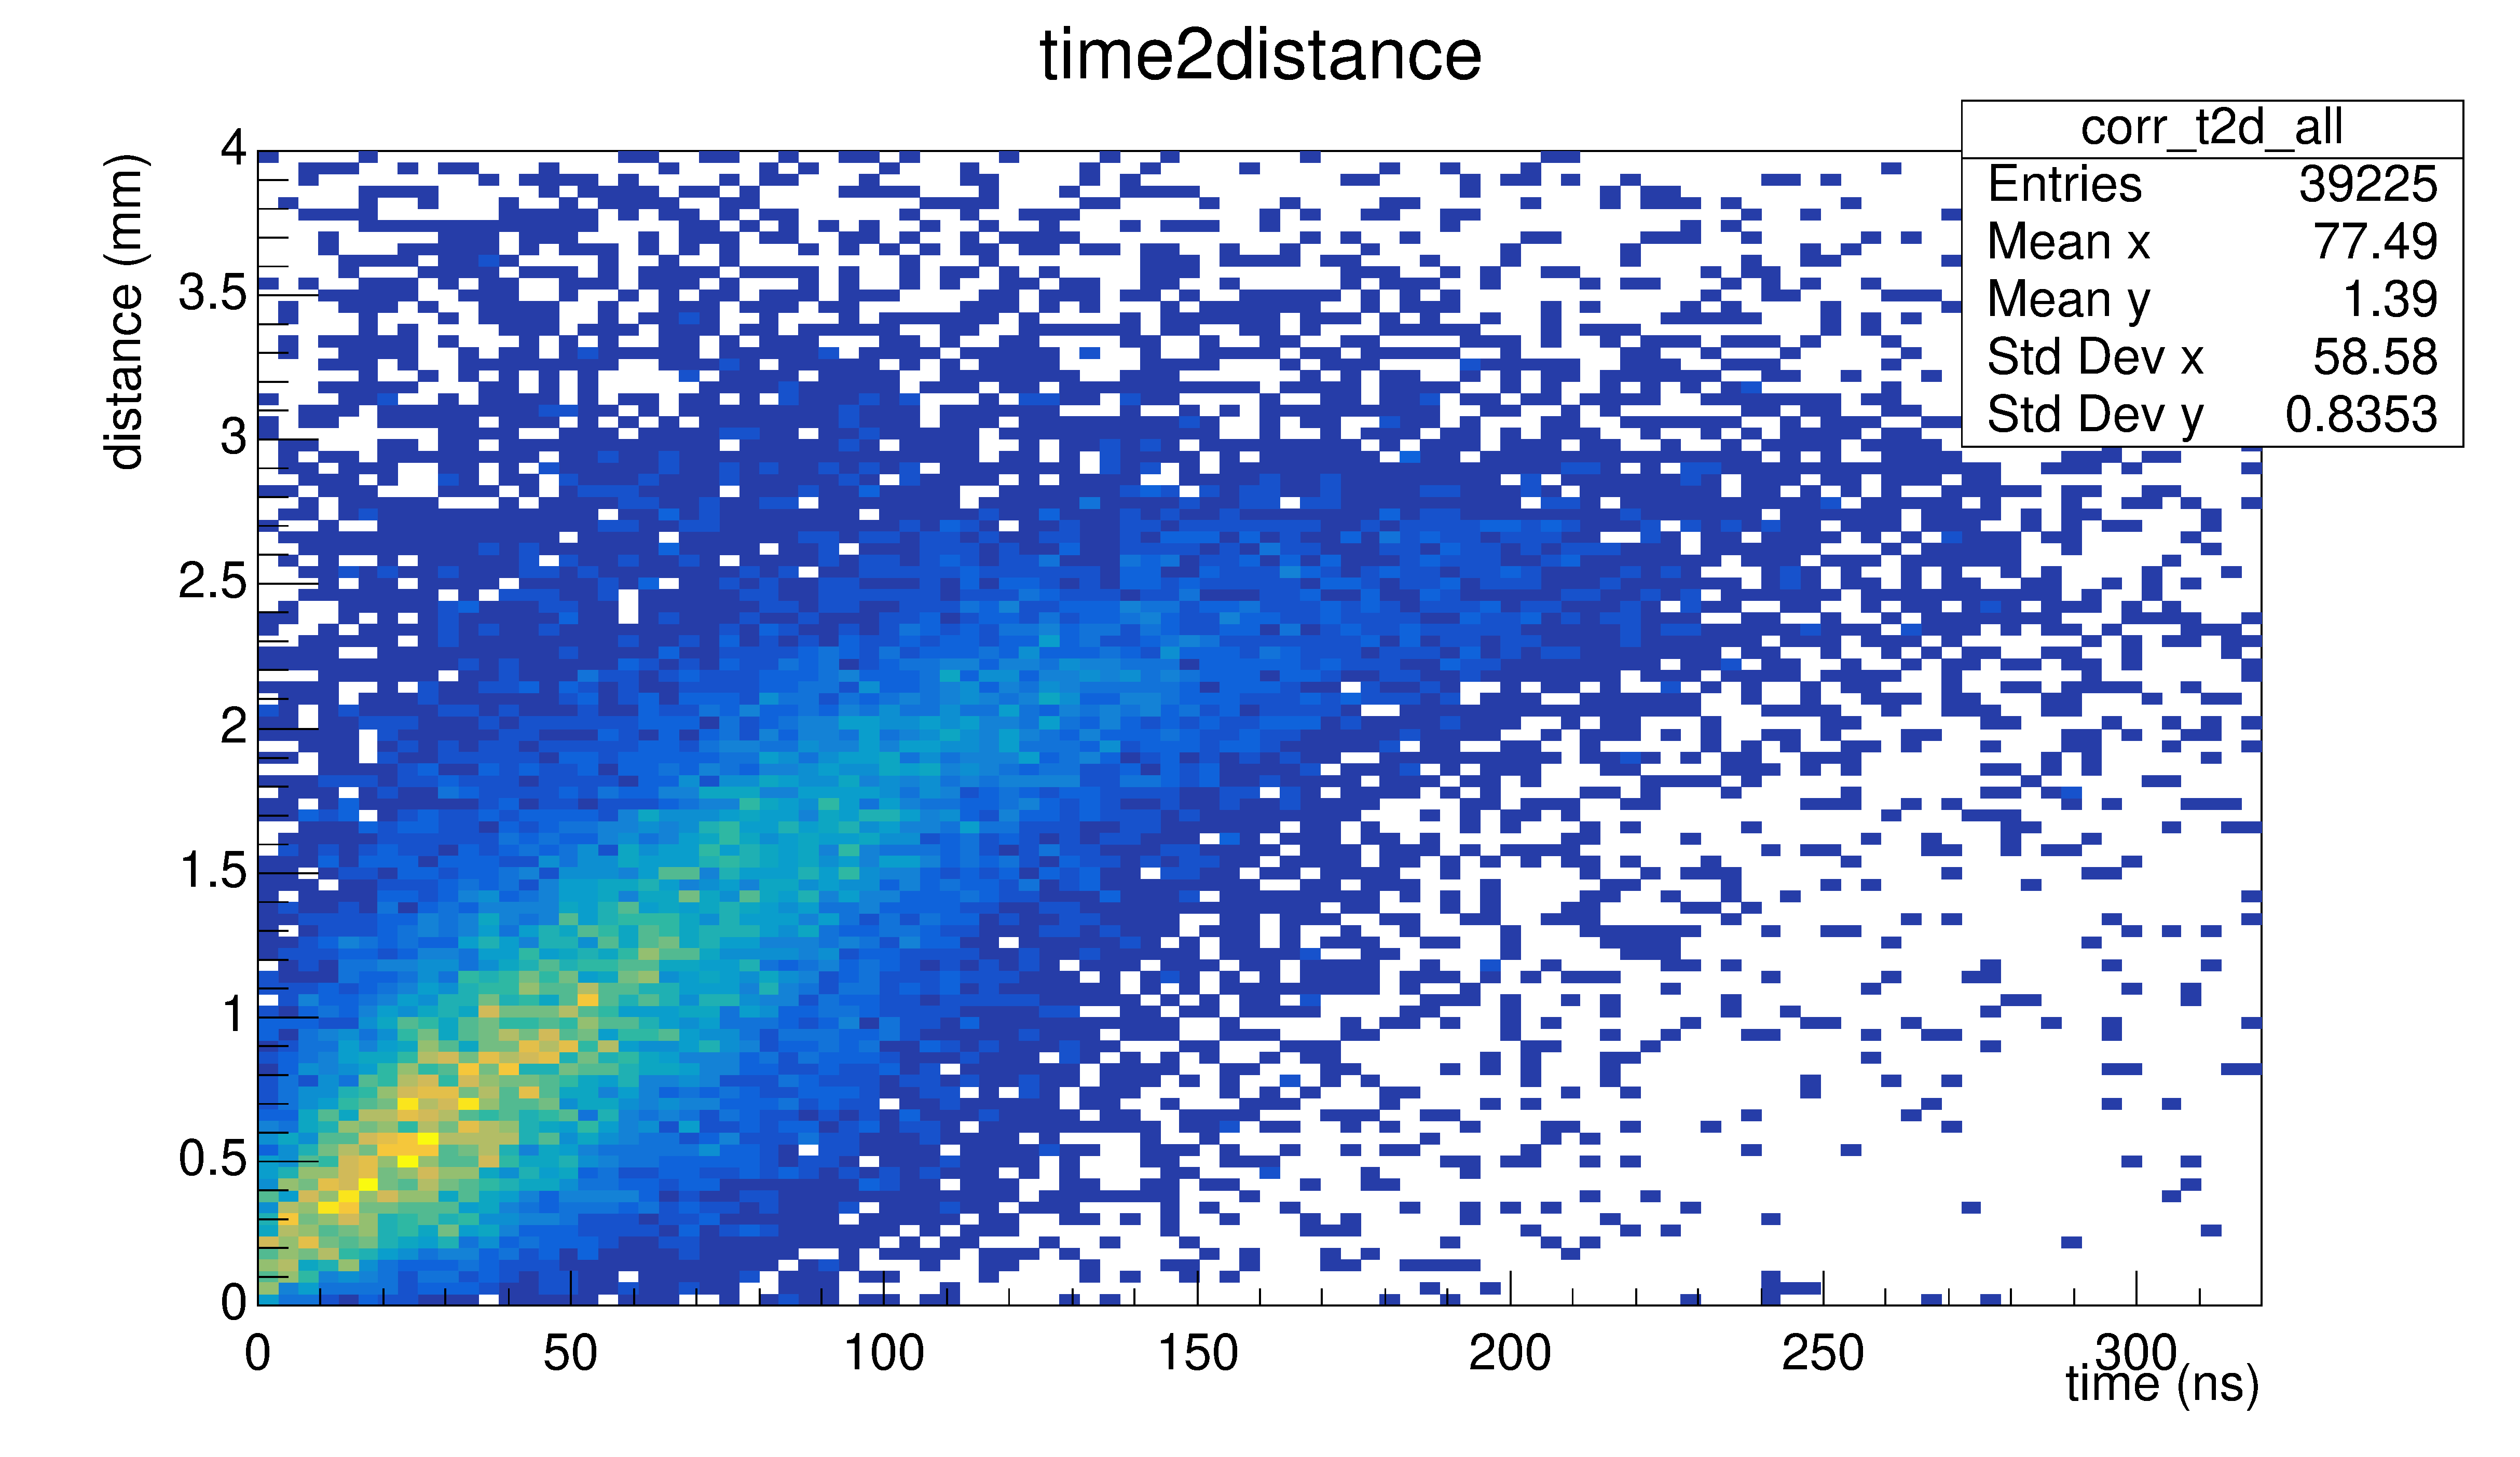
\includegraphics[width=0.45\linewidth]{figures/old_t2d.pdf} \\
    \end{tabular}
\end{frame}



\end{document}


